\documentclass[a4paper]{article}

\usepackage[spanish]{babel}
\usepackage{listings}
\usepackage[utf8]{inputenc}
\usepackage{titling}
\usepackage{enumitem}
\usepackage{fancyhdr}
\usepackage{xcolor}
\usepackage{geometry}
\usepackage{graphicx}
\geometry{a4paper, margin=7em}


\lstset{
    frame=single,
    breaklines=true,
    numbers=left,
    keywordstyle=\color{blue},
    numbersep=15pt,
    numberstyle=,
    basicstyle=\linespread{1.5}\selectfont\ttfamily,
    commentstyle=\color{gray},
    stringstyle=\color{orange},
    identifierstyle=\color{green!40!black},
}

%%\setlength{\parindent}{4em}
\setlength{\parindent}{0em}
%%\setlength{\parskip}{1em}
    
%%\renewcommand{\familydefault}{phv} %%Seleccionamos Helvetica
    
\lstdefinestyle{console}
{
    numbers=left,
    backgroundcolor=\color{violet},
    %%belowcaptionskip=1\baselineskip,
    breaklines=true,
    %%xleftmargin=\parindent,
    %%showstringspaces=false,
    basicstyle=\footnotesize\ttfamily,
    %%keywordstyle=\bfseries\color{green!40!black},
    %%commentstyle=\itshape\color{green},
    %%identifierstyle=\color{blue},
    %%stringstyle=\color{orange},
    basicstyle=\scriptsize\color{white}\ttfamily,
}
    
\title{Mapa de memoria}
\author{Aldán Creo Mariño}
    
    
\pagestyle{fancy}
\fancyfoot[R]{\thepage}
\fancyfoot[C]{}
\makeatletter
\let\runauthor\@author
\let\runtitle\@title
\makeatother
\fancyhead[L]{\runauthor}
\fancyhead[R]{\thesection}
    
\begin{document}
\maketitle

\section{Mapa de memoria}

El siguiente mapa de memoria se produce cuando enlazo dinámicamente:

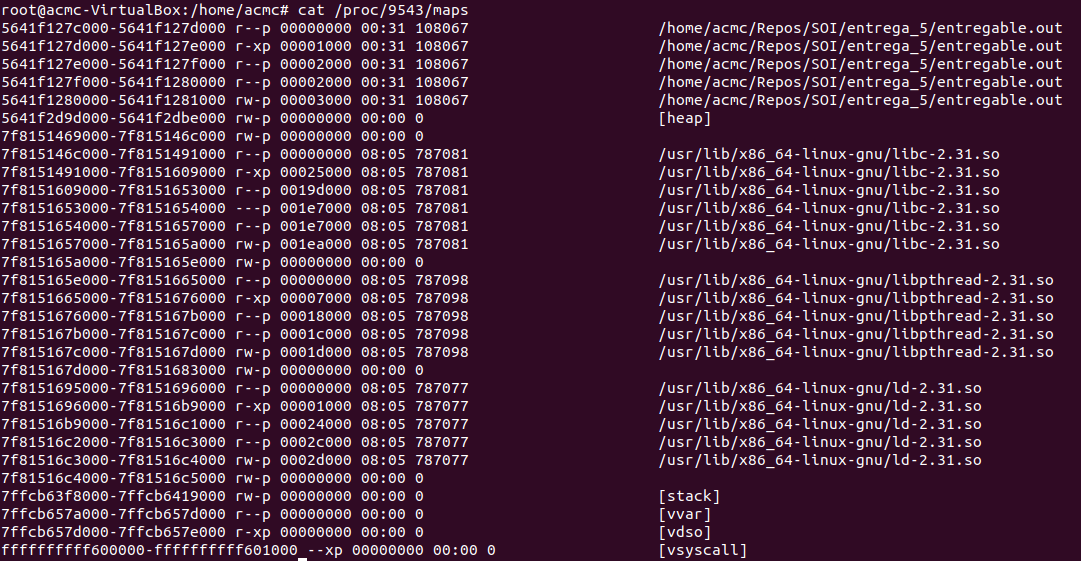
\includegraphics[scale=0.423]{6_padre.png}

\section{¿Dónde se guardan las variables?}

\subsection{Variables globales}

Las variables globales se guardan en el segmento de datos ({\ttfamily.data}, en el archivo de ensamblador), inicializadas o sin inicializar. En el mapa de memoria del proceso, corresponderán con la sección con permisos de lectura y escritura, pero no ejecución, que se mapea al archivo del código (línea 5).

\subsection{Variables locales}

Las variables locales se guardan en el stack. Cuando se entra en una función, el compilador de C incluye código para decrementar el puntero del stack, y reservar por tanto memoria para las variables locales a la función. Cuando se sale de la función concreta, se incrementa el puntero, ``liberando'' de forma efectiva esa memoria.

\subsection{Memoria dinámica}

La memoria dinámica es un concepto algo más abstracto. En general, podemos decir que se refiere a memoria mapeada en el proceso 

\begin{center}
\def\arraystretch{1.5}
\begin{tabular}{ | c | c | c | c | c | c | c | }
    \hline
     inicio & fin & permisos & desplazamiento & RELLENAR & RELLENAR &mapeo \\ \hline
     55fef1673000 & 55fef1674000 & r--p & 00000000 & 00:31 & 774 & /home/acmc/Repos/SOI/entrega\_5/a.out \\ \hline
55fef1674000 & 55fef1675000 & r-xp & 00001000 & 00:31 & 774 & /home/acmc/Repos/SOI/entrega\_5/a.out \\ \hline
55fef1675000 & 55fef1676000 & r--p & 00002000 & 00:31 & 774 & /home/acmc/Repos/SOI/entrega\_5/a.out \\ \hline
55fef1676000 & 55fef1677000 & r--p & 00002000 & 00:31 & 774 & /home/acmc/Repos/SOI/entrega\_5/a.out \\ \hline
55fef1677000 & 55fef1678000 & rw-p & 00003000 & 00:31 & 774 & /home/acmc/Repos/SOI/entrega\_5/a.out \\ \hline
55fef1f84000 & 55fef1fa5000 & rw-p & 00000000 & 00:00 & 0 & [heap] \\ \hline
7f99eef4b000 & 7f99eef70000 & r--p & 00000000 & 08:05 & 787081 & /usr/lib/x86\_64-linux-gnu/libc-2.31.so \\ \hline
7f99eef70000 & 7f99ef0e8000 & r-xp & 00025000 & 08:05 & 787081 & /usr/lib/x86\_64-linux-gnu/libc-2.31.so \\ \hline
7f99ef0e8000 & 7f99ef132000 & r--p & 0019d000 & 08:05 & 787081 & /usr/lib/x86\_64-linux-gnu/libc-2.31.so \\ \hline
7f99ef132000 & 7f99ef133000 & ---p & 001e7000 & 08:05 & 787081 & /usr/lib/x86\_64-linux-gnu/libc-2.31.so \\ \hline
7f99ef133000 & 7f99ef136000 & r--p & 001e7000 & 08:05 & 787081 & /usr/lib/x86\_64-linux-gnu/libc-2.31.so \\ \hline
7f99ef136000 & 7f99ef139000 & rw-p & 001ea000 & 08:05 & 787081 & /usr/lib/x86\_64-linux-gnu/libc-2.31.so \\ \hline
7f99ef139000 & 7f99ef13f000 & rw-p & 00000000 & 00:00 & 0 &  \\ \hline
7f99ef151000 & 7f99ef152000 & r--p & 00000000 & 08:05 & 787077 & /usr/lib/x86\_64-linux-gnu/ld-2.31.so \\ \hline
7f99ef152000 & 7f99ef175000 & r-xp & 00001000 & 08:05 & 787077 & /usr/lib/x86\_64-linux-gnu/ld-2.31.so \\ \hline
7f99ef175000 & 7f99ef17d000 & r--p & 00024000 & 08:05 & 787077 & /usr/lib/x86\_64-linux-gnu/ld-2.31.so \\ \hline
7f99ef17e000 & 7f99ef17f000 & r--p & 0002c000 & 08:05 & 787077 & /usr/lib/x86\_64-linux-gnu/ld-2.31.so \\ \hline
7f99ef17f000 & 7f99ef180000 & rw-p & 0002d000 & 08:05 & 787077 & /usr/lib/x86\_64-linux-gnu/ld-2.31.so \\ \hline
7f99ef180000 & 7f99ef181000 & rw-p & 00000000 & 00:00 & 0 &  \\ \hline
7fff40394000 & 7fff403b5000 & rw-p & 00000000 & 00:00 & 0 & [stack] \\ \hline
7fff403fa000 & 7fff403fd000 & r--p & 00000000 & 00:00 & 0 & [vvar] \\ \hline
7fff403fd000 & 7fff403fe000 & r-xp & 00000000 & 00:00 & 0 & [vdso] \\ \hline
ffffffffff600000 & ffffffffff601000 & --xp & 00000000 & 00:00 & 0 & [vsyscall] \\ \hline
\end{tabular}
\end{center}

\section{Ejercicio 4}
\section{Ejercicio 5}
871kB
16kB

\end{document}